%==============================================================================
% tento soubor pouzijte jako zaklad
% this file should be used as a base for the thesis
% Autoři / Authors: 2008 Michal Bidlo, 2016 Jaroslav Dytrych
% Kontakt pro dotazy a připomínky: dytrych@fit.vutbr.cz
% Contact for questions and comments: dytrych@fit.vutbr.cz
%==============================================================================
% kodovani: UTF-8 (zmena prikazem iconv, recode nebo cstocs)
% encoding: UTF-8 (you can change it by command iconv, recode or cstocs)
%------------------------------------------------------------------------------
% zpracování / processing: make, make pdf, make clean
%==============================================================================
% Soubory, které je nutné upravit: / Files which have to be edited:
%   projekt-20-literatura-bibliography.bib - literatura / bibliography
%   projekt-01-kapitoly-chapters.tex - obsah práce / the thesis content
%   projekt-30-prilohy-appendices.tex - přílohy / appendices
%==============================================================================
\documentclass[english]{fitthesis} % bez zadání - pro začátek práce, aby nebyl problém s překladem
%\documentclass[english]{fitthesis} % without assignment - for the work start to avoid compilation problem
%\documentclass[zadani]{fitthesis} % odevzdani do wisu - odkazy jsou barevné
%\documentclass[english,zadani]{fitthesis} % for submission to the IS FIT - links are color
%\documentclass[zadani,print]{fitthesis} % pro tisk - odkazy jsou černé
%\documentclass[zadani,cprint]{fitthesis} % pro barevný tisk - odkazy jsou černé, znak VUT barevný
%\documentclass[english,zadani,print]{fitthesis} % for the color print - links are black
%\documentclass[english,zadani,cprint]{fitthesis} % for the print - links are black, logo is color
% * Je-li práce psaná v anglickém jazyce, je zapotřebí u třídy použít 
%   parametr english následovně:
%   If thesis is written in english, it is necessary to use 
%   parameter english as follows:
%      \documentclass[english]{fitthesis}
% * Je-li práce psaná ve slovenském jazyce, je zapotřebí u třídy použít 
%   parametr slovak následovně:
%   If the work is written in the Slovak language, it is necessary 
%   to use parameter slovak as follows:
%      \documentclass[slovak]{fitthesis}
% * Je-li práce psaná v anglickém jazyce se slovenským abstraktem apod., 
%   je zapotřebí u třídy použít parametry english a enslovak následovně:
%   If the work is written in English with the Slovak abstract, etc., 
%   it is necessary to use parameters english and enslovak as follows:
%      \documentclass[english,enslovak]{fitthesis}

% Základní balíčky jsou dole v souboru šablony fitthesis.cls
% Basic packages are at the bottom of template file fitthesis.cls
% zde můžeme vložit vlastní balíčky / you can place own packages here
\usepackage{listings}

% Kompilace po částech (rychlejší, ale v náhledu nemusí být vše aktuální)
% Compilation piecewise (faster, but not all parts in preview will be up-to-date)
% \usepackage{subfiles}

% Nastavení cesty k obrázkům
% Setting of a path to the pictures
\graphicspath{{obrazky-figures/}{./obrazky-figures/}}
%\graphicspath{{obrazky-figures/}{../obrazky-figures/}}

%---rm---------------
\renewcommand{\rmdefault}{lmr}%zavede Latin Modern Roman jako rm / set Latin Modern Roman as rm
%---sf---------------
\renewcommand{\sfdefault}{qhv}%zavede TeX Gyre Heros jako sf
%---tt------------
\renewcommand{\ttdefault}{lmtt}% zavede Latin Modern tt jako tt

% vypne funkci šablony, která automaticky nahrazuje uvozovky,
% aby nebyly prováděny nevhodné náhrady v popisech API apod.
% disables function of the template which replaces quotation marks
% to avoid unnecessary replacements in the API descriptions etc.
\csdoublequotesoff

% =======================================================================
% balíček "hyperref" vytváří klikací odkazy v pdf, pokud tedy použijeme pdflatex
% problém je, že balíček hyperref musí být uveden jako poslední, takže nemůže
% být v šabloně
% "hyperref" package create clickable links in pdf if you are using pdflatex.
% Problem is that this package have to be introduced as the last one so it 
% can not be placed in the template file.
\ifWis
\ifx\pdfoutput\undefined % nejedeme pod pdflatexem / we are not using pdflatex
\else
  \usepackage{color}
  \usepackage[unicode,colorlinks,hyperindex,plainpages=false,pdftex]{hyperref}
  \definecolor{links}{rgb}{0.4,0.5,0}
  \definecolor{anchors}{rgb}{1,0,0}
  \def\AnchorColor{anchors}
  \def\LinkColor{links}
  \def\pdfBorderAttrs{/Border [0 0 0] }  % bez okrajů kolem odkazů / without margins around links
  \pdfcompresslevel=9
\fi
\else % pro tisk budou odkazy, na které se dá klikat, černé / for the print clickable links will be black
\ifx\pdfoutput\undefined % nejedeme pod pdflatexem / we are not using pdflatex
\else
  \usepackage{color}
  \usepackage[unicode,colorlinks,hyperindex,plainpages=false,pdftex,urlcolor=black,linkcolor=black,citecolor=black]{hyperref}
  \definecolor{links}{rgb}{0,0,0}
  \definecolor{anchors}{rgb}{0,0,0}
  \def\AnchorColor{anchors}
  \def\LinkColor{links}
  \def\pdfBorderAttrs{/Border [0 0 0] } % bez okrajů kolem odkazů / without margins around links
  \pdfcompresslevel=9
\fi
\fi
% Řešení problému, kdy klikací odkazy na obrázky vedou za obrázek
% This solves the problems with links which leads after the picture
\usepackage[all]{hypcap}

% Informace o práci/projektu / Information about the thesis
%---------------------------------------------------------------------------
\projectinfo{
  %Prace / Thesis
  project={BP},            %typ práce BP/SP/DP/DR  / thesis type (SP = term project)
  year={2019},             % rok odevzdání / year of submission
  date=\today,             % datum odevzdání / submission date
  %Nazev prace / thesis title
  title.cs={Výkonnostní testování plánovače linuxového kernelu},  % název práce v češtině či slovenštině (dle zadání) / thesis title in czech language (according to assignment)
  title.en={Performance Testing of Linux Kernel Scheduler}, % název práce v angličtině / thesis title in english
  title.length={13.2cm}, % nastavení délky bloku s titulkem pro úpravu zalomení řádku (lze definovat zde nebo níže) / setting the length of a block with a thesis title for adjusting a line break (can be defined here or below)
  %Autor / Author
  author.name={Jiří},   % jméno autora / author name
  author.surname={Vozár},   % příjmení autora / author surname 
  %author.title.p={Bc.}, % titul před jménem (nepovinné) / title before the name (optional)
  %author.title.a={Ph.D.}, % titul za jménem (nepovinné) / title after the name (optional)
  %Ustav / Department
  department={UITS}, % doplňte příslušnou zkratku dle ústavu na zadání: UPSY/UIFS/UITS/UPGM / fill in appropriate abbreviation of the department according to assignment: UPSY/UIFS/UITS/UPGM
  % Školitel / supervisor
  supervisor.name={Viktor},   % jméno školitele / supervisor name 
  supervisor.surname={Malík},   % příjmení školitele / supervisor surname
  supervisor.title.p={Ing.},   %titul před jménem (nepovinné) / title before the name (optional)
  %supervisor.title.a={},    %titul za jménem (nepovinné) / title after the name (optional)
  % Klíčová slova / keywords
  keywords.cs={Linux, jádro, plánovač úloh, CFS, testování, měření výkonu, vizualiace, strojové učení}, % klíčová slova v českém či slovenském jazyce / keywords in czech or slovak language
  keywords.en={Linux, kernel, task scheduler, CFS, testing, performance measurement, visualization, machine learning}, % klíčová slova v anglickém jazyce / keywords in english
  % Abstrakt / Abstract
  abstract.cs={Do tohoto odstavce bude zapsán výtah (abstrakt) práce v českém (slovenském) jazyce.}, % abstrakt v českém či slovenském jazyce / abstract in czech or slovak language
  abstract.en={Do tohoto odstavce bude zapsán výtah (abstrakt) práce v anglickém jazyce.}, % abstrakt v anglickém jazyce / abstract in english
  %abstract.en={An abstract of the work in English will be written in this paragraph.},
  % Prohlášení (u anglicky psané práce anglicky, u slovensky psané práce slovensky) / Declaration (for thesis in english should be in english)
%   declaration={Prohlašuji, že jsem tuto bakalářskou práci vypracoval samostatně pod vedením pana X...
% Další informace mi poskytli...
% Uvedl jsem všechny literární prameny a publikace, ze kterých jsem čerpal.},
  declaration={Hereby I declare that this bachelor's thesis was prepared as an original author’s work under the supervision of Mr. X
The supplementary information was provided by Mr. Y
All the relevant information sources, which were used during preparation of this thesis, are properly cited and included in the list of references.},
  % Poděkování (nepovinné, nejlépe v jazyce práce) / Acknowledgement (optional, ideally in the language of the thesis)
%   acknowledgment={V této sekci je možno uvést poděkování vedoucímu práce a těm, kteří poskytli odbornou pomoc
% (externí zadavatel, konzultant, apod.).},
  acknowledgment={Here it is possible to express thanks to the supervisor and to the people which provided professional help
(external submitter, consultant, etc.).},
  % Rozšířený abstrakt (cca 3 normostrany) - lze definovat zde nebo níže / Extended abstract (approximately 3 standard pages) - can be defined here or below
  %extendedabstract={Do tohoto odstavce bude zapsán rozšířený výtah (abstrakt) práce v českém (slovenském) jazyce.},
  %faculty={FIT}, % FIT/FEKT/FSI/FA/FCH/FP/FAST/FAVU/USI/DEF
  faculty.cs={Fakulta informačních technologií}, % Fakulta v češtině - pro využití této položky výše zvolte fakultu DEF / Faculty in Czech - for use of this entry select DEF above
  faculty.en={Faculty of Information Technology}, % Fakulta v angličtině - pro využití této položky výše zvolte fakultu DEF / Faculty in English - for use of this entry select DEF above
  department.cs={Ústav matematiky}, % Ústav v češtině - pro využití této položky výše zvolte ústav DEF nebo jej zakomentujte / Department in Czech - for use of this entry select DEF above or comment it out
  department.en={Institute of Mathematics} % Ústav v angličtině - pro využití této položky výše zvolte ústav DEF nebo jej zakomentujte / Department in English - for use of this entry select DEF above or comment it out
}

% Rozšířený abstrakt (cca 3 normostrany) - lze definovat zde nebo výše / Extended abstract (approximately 3 standard pages) - can be defined here or above
\extendedabstract{Do tohoto odstavce bude zapsán výtah (abstrakt) práce v českém (slovenském) jazyce.}

% nastavení délky bloku s titulkem pro úpravu zalomení řádku - lze definovat zde nebo výše / setting the length of a block with a thesis title for adjusting a line break - can be defined here or above
%\titlelength{14.5cm}


% řeší první/poslední řádek odstavce na předchozí/následující stránce
% solves first/last row of the paragraph on the previous/next page
\clubpenalty=10000
\widowpenalty=10000

\begin{document}
  % Vysazeni titulnich stran / Typesetting of the title pages
  % ----------------------------------------------
  \maketitle
  % Obsah
  % ----------------------------------------------
  \setlength{\parskip}{0pt}

  {\hypersetup{hidelinks}\tableofcontents}
  
  % Seznam obrazku a tabulek (pokud prace obsahuje velke mnozstvi obrazku, tak se to hodi)
  % List of figures and list of tables (if the thesis contains a lot of pictures, it is good)
  \ifczech
    \renewcommand\listfigurename{Seznam obrázků}
  \fi
  \ifslovak
    \renewcommand\listfigurename{Zoznam obrázkov}
  \fi
  % \listoffigures
  
  \ifczech
    \renewcommand\listtablename{Seznam tabulek}
  \fi
  \ifslovak
    \renewcommand\listtablename{Zoznam tabuliek}
  \fi
  % \listoftables 

  \ifODSAZ
    \setlength{\parskip}{0.5\bigskipamount}
  \else
    \setlength{\parskip}{0pt}
  \fi

  % vynechani stranky v oboustrannem rezimu
  % Skip the page in the two-sided mode
  \iftwoside
    \cleardoublepage
  \fi

  % Text prace / Thesis text
  % ----------------------------------------------
  \chapter{Introduction}
Performance of operating system is crucial, because it can significantly affect all the applications running above it.
When a regression in new version occurs, business applications can be even financially affected.

Scheduler was simple. Multi-core CPUs made the scheduler little more complex, but those complications were tuned through time.
Next milestone was introduction of multi-CPU machines with separated memory for each physical unit.

Compared to functional testing, performance isn't evaluated as true/false result, but relative change to previous measurement.
Due to this complexity is hard to use common tools for inspecting performance.
The biggest regression in scheduler doesn't hide in uneffective code, but in wrong placement of processes to cores and it's queues.

The usual testing method is simulating load simmilar to real usage.
To achieve this there are many benchmarks targetting different types of load, usually many parallel process, sometimes communicating between each other.

Good performance tests usually create great amount of data, which is required to be processed, aggregaed and visualised.

\chapter{Linux process scheduling}
Scheduler is a part of an operating system which assigns the processor time to tasks.
Its main goal is to maximize effectivity of the CPU usage and fairness of assigned
CPU time to each task.

There are two opposing targets for a scheduler - either maximazing throughput or
minimizing latency. Lower amount of context switches leaves more CPU time for
applications, but raises the response time on system events.
While user's workstation aims for a low response time, computational servers
require high throughput. Scheduler can be usually tuned to fit the intended
purpose.

\section{Completely Fair Scheduler}
Completely Fair Scheduler is the current Linux process scheduler, which was
merged into the version
2.6.23 of the Linux kernel in 2007. Its author is Ingo Molnár, who is author of previous
O(1) scheduler as well.

It features queuing tasks in a red-black tree structure ordered by the time spent
running on the CPU so far. Red-black tree is a binary search
tree with self-balancing mechanism based on marking nodes with either red or
black color.
When the scheduler needs to choose the next task to run, it
takes the leftmost node with the lowest execution time. 

The time complexity of the CFS scheduling is O(log N). Taking the leftmost node with
the next task can be done in a constant time, but queuing the task again requires
O(log N) operations to insert it back into the red-black tree. Even with the
higher scheduling complexity, the CFS scheduler has better fairness and
responsiveness than with O(1) scheduler, which used simple queue to choose the
next task.

On multi-core systems scheduler uses separate queue for each core. To effectivly
use the processing power, scheduler must regularly balance those queues by
moving processes from the most busy cores to idle ones.

When moving processes between cores scheduler takes in account topology of the
system. Loosing data from caches after migration can have a bigger impact on
performance, than leaving the process on the busy core.

\section{NUMA}
With an increasing amount of cores and arrival of the multi-socket machines
appeared problems with bus bandwidth between CPUs and their common memory. This
problem was solved with \emph{Non-Uniform Memory Access} (NUMA) technology.
Each processor or group of cores has its own memory and bus. This allows higher
access speed to the local memory of the processor, than on UMA systems with
common bus. However, accesing memory from other nodes is more expensive. The
data must be transfered through interconnect bus or even controller, which slows
the system significantly.

% TODO cite http://highscalability.com/blog/2013/5/30/google-finds-numa-up-to-20-slower-for-gmail-and-websearch.html
Access to memory on another node or even moving the data is expensive and with
wrong approach can cause worse performance, than Unified memory access systems.
Balancing processes between NUMA nodes is still in active development, which
brings many changes both to better or sometimes worse performance.


\chapter{Performance measurement}
A basic way to measure performance of system is benchmark. They return some numbers representing throughput of system, but can't tell more about the system behavior.
To get a better insight on the system, there are many performance analysis tools to observe cpu and memory utilization, location of processes on cores or their time out of cpu.
\texttt{http://www.brendangregg.com/activebenchmarking.html}

\section{Benchmarks}

\subsection{NAS Parallel Benchmarks}
NAS Parallel Benchmarks is set of benchmarks focused on performance of highly
parallel computations on supercomputers. In addition to floating point
computations it targets communication and data movement between computation
nodes. Performed algorithms are based on large scale computational fluid
dynamics at the Numerical Aerodynamic Simulation (NAS) Program which is based at
NASA Ames Research Center.

Benchmarks are written in Fortran-90 or C language, beacause they were the most
commonly used programming languages in scientific parallel computing community
by the time they were created. They can be compiled with different classes of
problem sizes to suit machines with different amount of memory and computational
power.

Many parameters can be passed to benchmark also before execution to tweak
properties of behavior. One of them is number of computation thread, which in
lower amount slowers the run time, but allows to measure behavior of system
without full usage.

\begin{figure}
  \centering
  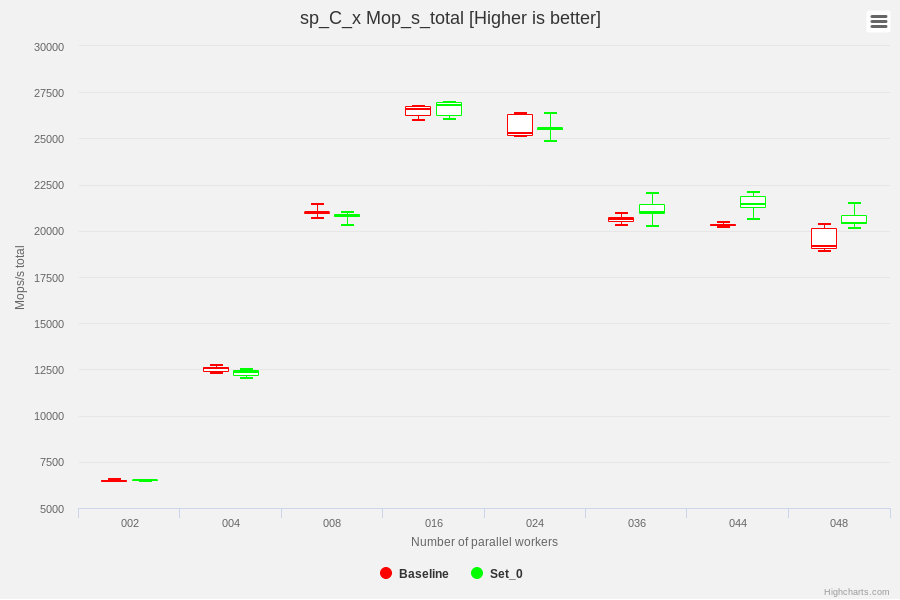
\includegraphics[width=10cm]{obrazky-figures/nas}
  \caption{Example of Scalar Penta-diagonal solver results from NAS Parallel with
  different number of computational threads.}
\end{figure}

\subsection{SPECjbb2005}
Java Business Benchmark behaves as a server-side Java application. It is primarily focused on measuring performance of Java implementation, but also reflects performance of operating system and cpu itself.
It models system of wholesale company as a multitier application. The benchmark
itself creates the load, measures the throughput and also generates simple
report in HTML and raw text formats.

The main output value is \emph{throughput} in units called \emph{SPECjbb2005
  bops} \footnote{Business operations per second}.
In case of using more JVM instances, there is a second unit called SPECjbb2005
bops/JVM representing average throughput of single JVM\footnote{Java virtual machine} instance.
Another collected metric is memory comsumption, which isn't that useful in
scheduler performance monitoring.

\subsection{LINPACK benchmark}
LINPACK Benchmark comes from LINPACK package, wich was used to solve systems of linear equations in single or double precision.

\subsection{Stream benchmark}

\section{Performance analysis tools}

\subsection{time}
Simple command, that can measure resource usage. Usually it's used to measure
running time of process.

It isn't bash builtin, but programm, that must be usually called from /usr/bin/time.

\subsection{ps}
This command lists current processes with information about them. In
\texttt{PSR} and \texttt{NUMA} column are useful informations of CPU and NUMA
node number, where is the process running.

\subsection{mpstat}

\subsection{turbostat}
This tool provides measuring of CPU usage and mainly its frequency.

\subsection{perf}


\chapter{Storing the results}
Benchmarks usually generate long human-readable output in text or even HTML
format. This is useful when analyzing single report. In the output are details
of the test run itself, simple resource usage or success of result validation.
However, the amount of result starts to rise with repeated runs, different
amount of instances and new versions kernels.

For the comparison of performance results, it is usually enough the number
representing throughput or time of each benchmark run. Those numbers can be
preprocessed from the benchmark output files to a format more suitable for quick
accesing required data.

\section{XML files}
XML is markup language, that can store heterogeneous data in tree structure.
However, the main feature of this format is human-readability. Even with the
inefficient storage of numerical data and repetition of tag and attribute names,
it allows user to quicky see the numbers without any processing of the data.

\section{Database}


\chapter{Displaying the results}

\section{Heatmaps}

\section{Boxplots}
Boxplot is method for displaying statistical properties of data groups. The
usually displayed values are minimum, 1\textsuperscript{st} quartile, median,
3\textsuperscript{rd} quartile and maximum.
This feature is useful to visualize accuaracy and reliability of measurement.
Then it's easier to distinguish performance regression from noise.

\begin{figure}
  \centering
  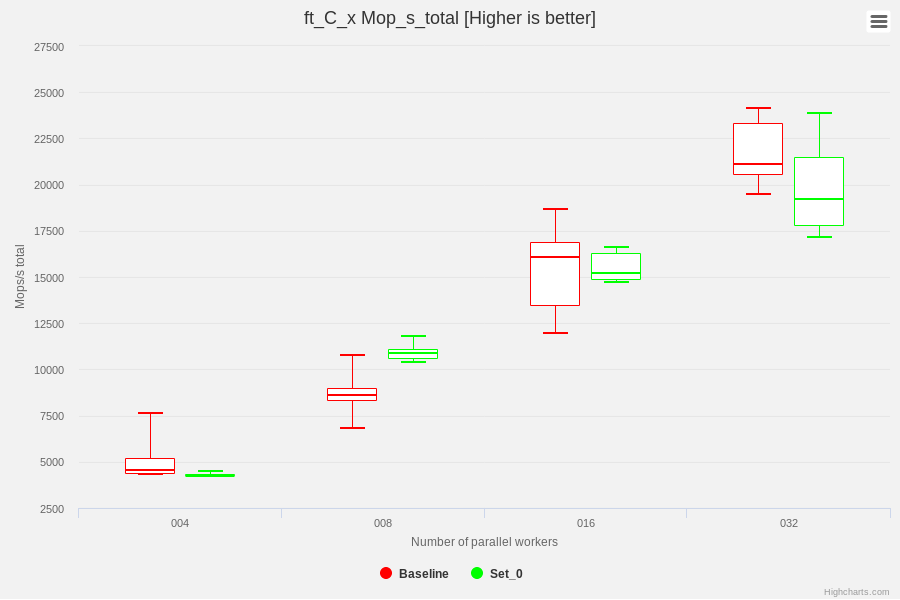
\includegraphics[width=12cm]{obrazky-figures/boxplot}
  \caption{Example of boxplot showing Mops of NAS benchmark with different
    number of threads}
\end{figure}


\chapter{Timelines}
An common way to get performance report is to compare two results. Usually, they
are called baseline and target results. The comparison of two results allows to
write many details about the measurement and changes between versions. Those
details usually contain clues to the cause of possible performance change.

However, sometimes is not enough to compare just two versions and larger amount
of results over longer period of time can bring a new perspective. There is much
more visible difference between the deviation from measurement error and the
performance change. It is also easier to find the versions, where a
performance degradation occured and where was fixed.

With larger amount of data, there can also emerge performance drops, which
appeared continuously over longer period of time and couldn't be spotted,
because they were in tolerance due to deviation.

\section{Result storage}
Benchmark results are stored on filesystem in directories. Each result consists
of two XML files with information and preprocessed main data from the test run,
more files with larger complementary data from analysis tools and compressed
original outputs from benchmark. First XML file contains metadata from the test
run including time, machine hostname, kernel and OS version, benchmark name,
configuration of environment, which could affect the result and few other data.
The second XML file contains the important preprocessed data itself.

The program has to go throgh all these results to choose the right ones for the
following creation of graphs.

\section{Comparison rules}
For automatic report generation are essential rules, which will specify results,
that can be used and in which role. I chose \emph{regular expressions} to match
properties of results. Regular expressions offer broad possibilities to describe
shape of kernel version or just value of any evironment configuration. To filter
all builds of kernel 4.18 works simple pattern \texttt{kernel-4.18\textbackslash
..*}.

To store the rules are stored in XML file with same node naming as in XML file
with result properties. The first level of XML document contains three nodes
representing purpose of rules.
\begin{itemize}
  \item \textbf{Baseline rules} specify the first result in plotted set. Acts as
    main result others are compared to.
  \item \textbf{Target rules} define the results to be plotted.
  \item \textbf{Starting rules} are for case, when base result is not from
    target set of results and specifying first target result with regex would be
    hard.
\end{itemize}
Each of theese nodes then contain in them nodes with the rules.


\chapter{Automatic evaluation}
With every expansion of regular kernel testing rises the amount of produced
results. With more machines with different configurations, benchmarks with
different focus or baselines from different supported versions, number of results
can rise with every new kernel version even by hundrets. This tends to automate
the repetitive classification of results between pass and fail to leave results
without significant change and focus on the ones with performance regressions.

\section{Marking of results}
To teach automatic classificator is essential large amount of data. To reduce
time spent on marking of the passed and failed results I created a form in
report to quicken this process.

On machine for storing results is running simple server application for
commiting requests from the form. The server is written in Python built on top
of Flask framework. On request it finds given result and modifies its file with
marking for learning.

\begin{figure}
  \centering
  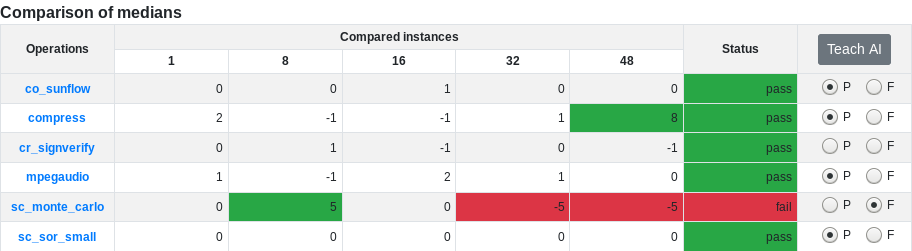
\includegraphics[width=12cm]{obrazky-figures/teaching_table}
  \caption{Form from HTML comparison report page to mark data for machine learning}
\end{figure}


%\chapter{Future work}


\chapter{Notes}
\begin{verbatim}
Linux scheduler
    CFS
    numa planning
        not easy for scheduler
        manual pinning option
            numactl
        group imbalance bug
    tune profiles
        focus on throughput or latency
Performance
    performance isn't simple pass/fail
    comparison of baseline and target kernel
    running just benchmark is waste of testing potential, it's good to collect more data
        http://www.brendangregg.com/activebenchmarking.html
    provisioning of machines with Beaker
    collecting system load data
        mpstat
            usage of every cpu
        numastat
        numatop
            usage of cpu and memory on each node
        ps
            psr and numa column
            cpu time
        time
            total, user and system time spent
        turbostat
        perf stat
        lstopo for hardware schema image
        free
    benchmarks
        specjbb2005
        specjvm2008
        nas parallel
        linpack benchmark
        stream (memory throughput)
        specjbb2015 - not stable
        hackbench - not tried yet
    scenarios
        variable number of benchmark instances
        with and without pinning processes to specific numa nodes
    result storing
        preprocessing to xml
        storing to database
        aggregating results
        computing statistical data
    plotting
        lstopo for plotting hardware topology
        bargraphs to show inaccuaracy
            operations per second (runtime of benchmark)
            time out of cpu
        detailed comparsion of two results
        timeline with many results over longer period of time
        heatmaps for core usage over time
            http://www.brendangregg.com/HeatMaps/utilization.html
        graph of process migration between numa nodes
Timelines
    analysis
    used technologies
    desing
    implementation
    output
Automatic regression detection
    motivation
    marking data
    preprocessing for classificator
    methods
        linear logistic regression
        decision trees
    evaluation
\end{verbatim}

\chapter{Specification}
\begin{enumerate}
\item Get acquainted with the existing methods for measuring performance of the Linux kernel scheduler and with means of storing of benchmarks results for further processing.
\item Study possible ways of processing these results with a focus on graphic interpretation and on methods for detection of performance degradation.
\item Design and implement a method for efficient graphic interpretation of long-term measurements.
\item Design and implement a method for automatic detection of performance regression.
\item Demonstrate the functionality of your implementation on at least two versions of the Linux kernel.
\item Evaluate the obtained results and discuss possibilities of further development of the project, especially of the automatic detection of performance regression.
\end{enumerate}

Literature:
\begin{itemize}
\item Lozi, Jean-Pierre, et al. "The Linux scheduler: a decade of wasted cores." Proceedings of the Eleventh European Conference on Computer Systems. ACM, 2016.
\item Daniel, P., and Cesati Marco. "Understanding the Linux kernel." (2007).
\item Bailey, David H., et al. "The NAS parallel benchmarks." The International Journal of Supercomputing Applications 5.3 (1991): 63-73.
\end{itemize}

  
  % Kompilace po částech (viz výše, nutno odkomentovat)
  % Compilation piecewise (see above, it is necessary to uncomment it)
  %\subfile{projekt-01-uvod-introduction}
  % ...
  %\subfile{chapters/projekt-05-conclusion}


  % Pouzita literatura / Bibliography
  % ----------------------------------------------
\ifslovak
  \makeatletter
  \def\@openbib@code{\addcontentsline{toc}{chapter}{Literatúra}}
  \makeatother
  \bibliographystyle{bib-styles/slovakiso}
\else
  \ifczech
    \makeatletter
    \def\@openbib@code{\addcontentsline{toc}{chapter}{Literatura}}
    \makeatother
    \bibliographystyle{bib-styles/czechiso}
  \else 
    \makeatletter
    \def\@openbib@code{\addcontentsline{toc}{chapter}{Bibliography}}
    \makeatother
    \bibliographystyle{bib-styles/englishiso}
  %  \bibliographystyle{alpha}
  \fi
\fi
  \begin{flushleft}
  \bibliography{projekt-20-literatura-bibliography}
  \end{flushleft}

  % vynechani stranky v oboustrannem rezimu
  % Skip the page in the two-sided mode
  \iftwoside
    \cleardoublepage
  \fi

  % Prilohy / Appendices
  % ---------------------------------------------
  \appendix
\ifczech
  \renewcommand{\appendixpagename}{Přílohy}
  \renewcommand{\appendixtocname}{Přílohy}
  \renewcommand{\appendixname}{Příloha}
\fi
\ifslovak
  \renewcommand{\appendixpagename}{Prílohy}
  \renewcommand{\appendixtocname}{Prílohy}
  \renewcommand{\appendixname}{Príloha}
\fi
%  \appendixpage

% vynechani stranky v oboustrannem rezimu
% Skip the page in the two-sided mode
%\iftwoside
%  \cleardoublepage
%\fi
  
\ifslovak
%  \section*{Zoznam príloh}
%  \addcontentsline{toc}{section}{Zoznam príloh}
\else
  \ifczech
%    \section*{Seznam příloh}
%    \addcontentsline{toc}{section}{Seznam příloh}
  \else
%    \section*{List of Appendices}
%    \addcontentsline{toc}{section}{List of Appendices}
  \fi
\fi
  \startcontents[chapters]
  \setlength{\parskip}{0pt}
  % seznam příloh / list of appendices
  % \printcontents[chapters]{l}{0}{\setcounter{tocdepth}{2}}
  
  \ifODSAZ
    \setlength{\parskip}{0.5\bigskipamount}
  \else
    \setlength{\parskip}{0pt}
  \fi
  
  % vynechani stranky v oboustrannem rezimu
  \iftwoside
    \cleardoublepage
  \fi
  
  % Přílohy / Appendices
  % Tento soubor nahraďte vlastním souborem s přílohami (nadpisy níže jsou pouze pro příklad)
% This file should be replaced with your file with an appendices (headings below are examples only)

% Umístění obsahu paměťového média do příloh je vhodné konzultovat s vedoucím
% Placing of table of contents of the memory media here should be consulted with a supervisor
%\chapter{Obsah přiloženého paměťového média}

%\chapter{Manuál} % manual

%\chapter{Konfigurační soubor} % Configuration file

%\chapter{RelaxNG Schéma konfiguračního souboru} % Scheme of RelaxNG configuration file

%\chapter{Plakát} % poster

\chapter{How to use this template}
\label{how}

This chapter describes the individual parts of the template, which is followed by instructions on how to use this template.

This version of the template is only temporary. The new one is going to be published by the end of the year 2017 and it will contain new instructions on how to properly use the template, obligatory instructions on how to work on bachelor's and master's thesis (recapitulation of instructions which are available online) and non-obligatory recommendations by some from the selected supervisors that are already available on-line (see links in literature file). The only files that will contain changes in the new version are \texttt{projekt-01-kapitoly-chapters.tex} and \texttt{projekt-30-prilohy-appendices.tex}. Content of each will be removed by every student and its content will be replaced by their own. The template is thus ready to be used even in the current version.\cite{fitWeb}

  
  % Kompilace po částech (viz výše, nutno odkomentovat)
  % Compilation piecewise (see above, it is necessary to uncomment it)
  %\subfile{projekt-30-prilohy-appendices}
  
\end{document}
